\documentclass{IFES-beamer}

% --------------------------------------------------- %
%                  Presentation info	              %
% --------------------------------------------------- %
\title[Presentation Template]{CONSTRUINDO UM PERFIL DO CONSUMO ENERGÉTICO DE ALGORITMOS EM UMA PLATAFORMA EMBARCADA } 
\author{Mayanna Rodrigues Ferreira}
\institute[IFCE]{
  Instituto Federal do Ceará\\
  Maracananu
}
\date{10 de Agosto de 2020}
\logo{
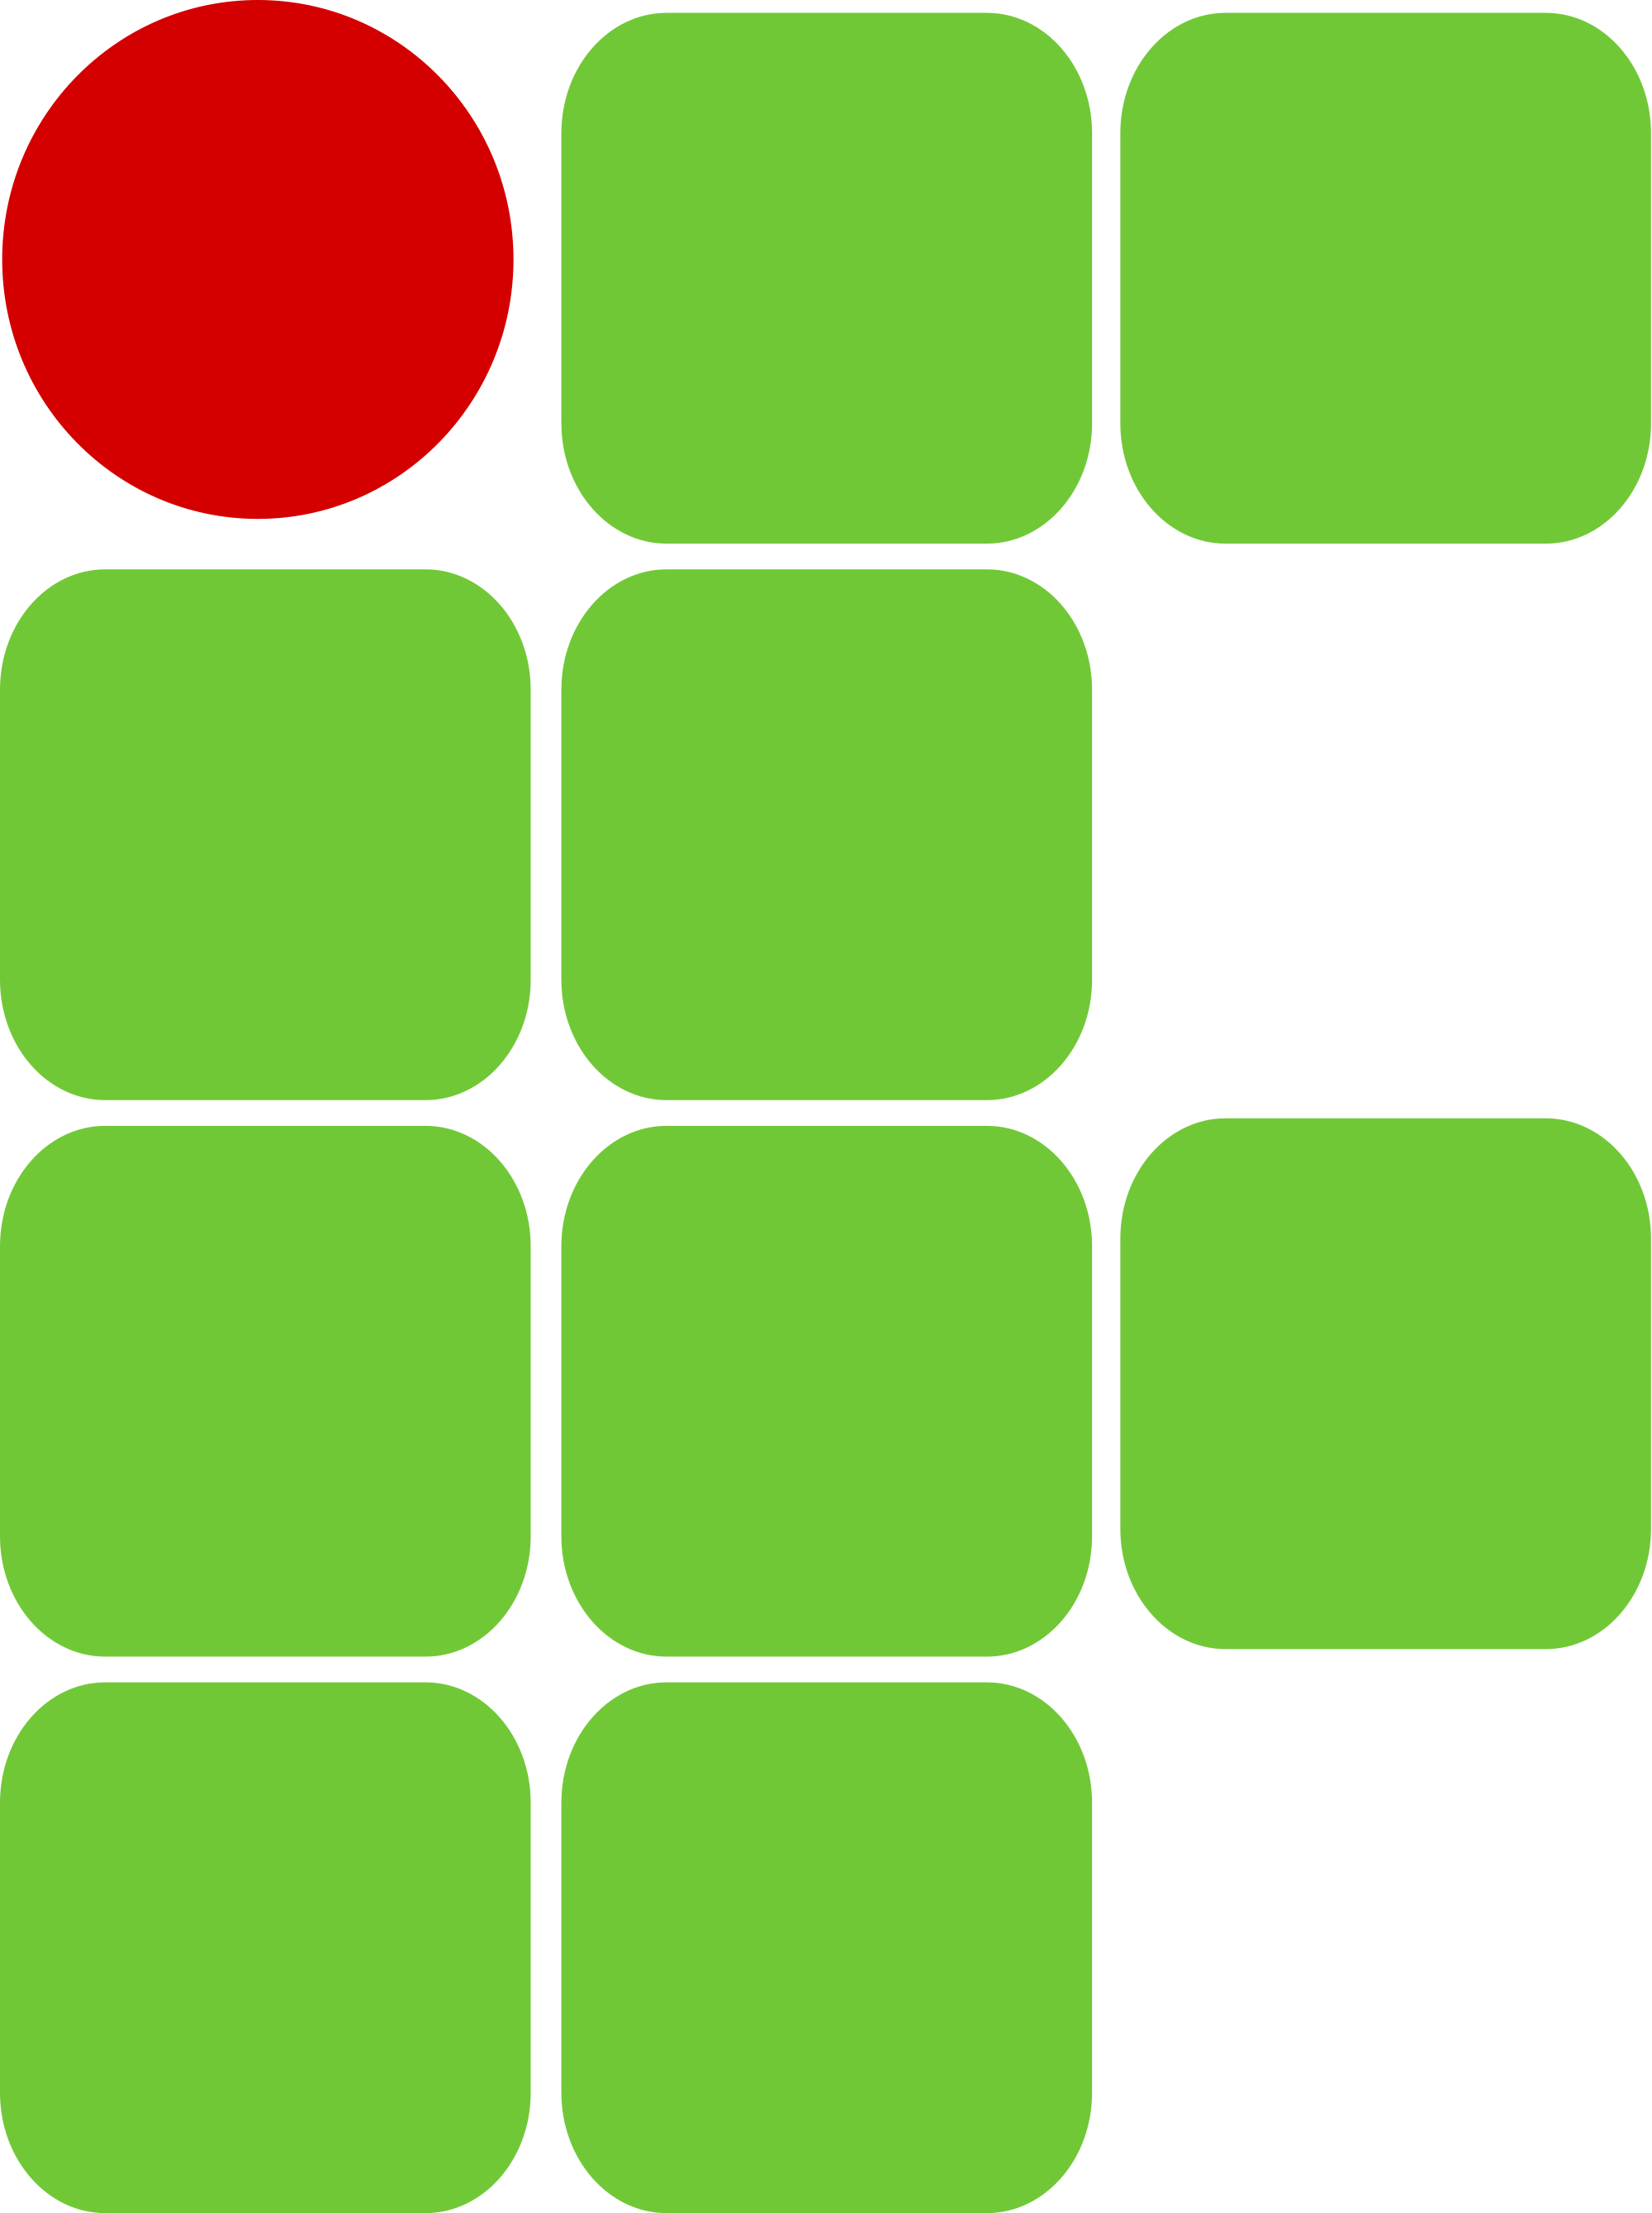
\includegraphics[scale=0.008]{images/logo.png}
}
\subject{Presentation subject} % metadata

% --------------------------------------------------- %
%                    Title + Schedule                 %
% --------------------------------------------------- %

\begin{document}

\begin{frame}
  \titlepage
\end{frame}

\begin{frame}{Sumário}
  \tableofcontents
\end{frame}

% --------------------------------------------------- %
%                      Presentation                   %
% --------------------------------------------------- %
\section{Introdução}
\begin{frame}{Introdução}
A tecnologia está cada vez mais presente na vida da sociedade atual. As evoluções dessas tecnologias nas últimas décadas foram enormes. Hoje, elas estão presentes em diversos âmbitos da sociedade, como na agricultura, no comércio, nos equipamentos médicos, no monitoramento de rodovias, nas casas e até no corpo humano. Nesse cenário, os sistemas embarcados tornam-se cada vez mais presentes no cotidiano.

\end{frame}
\begin{frame}{Motivação}

Diante da proeminente proliferação dos sistemas embarcados na sociedade e de todos os desafios existentes para torná-los mais eficientes quanto ao consumo energético, torna-se necessário ter conhecimento do perfil energético de determinados algoritmos que nos dispositivos serão utilizados.

\end{frame}

\begin{frame}{Objetivos}
\begin{block}{Objetivo Geral}
\begin{itemize}
  \item Traçar, de forma consistente, um perfil de consumo de energia de alguns algoritmos em um sistema embarcado em diferentes situações, permitindo, assim, uma avaliação apurada para uso em plataformas de si
\end{itemize}
\end{block}

\begin{block}{Objetivos Especificos}
\begin{itemize}
  \item Utilizar a plataforma apresentada no artigoAn FPGA-based evaluation platformfor energy harvesting embedded systems(ALCÂNTARA; DE LIMA; FURTADO,2019) para fazer os experimentos;
  \item Empregar os perfis de consumo de energia gerados em diferentes condições, para uso como fonte de dados para simulações;
  \item Comparar os perfis de consumo de um mesmo algoritmo em diferentes condições.
\end{itemize}
\end{block}
\end{frame}


\section{Fundamentação Teórica}
\begin{frame}{Fundamentação Teórica}
O gráfico mostra uma projeção de crecimento do IoT nos proximos anos.

\begin{figure}
\centering
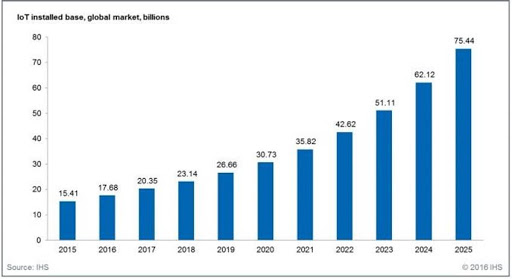
\includegraphics[width=\linewidth]{images/grafico.jpg}
\caption{ Figura 1 - The IoT market will be massive. Fonte IHS (2016) }
\end{figure}

\end{frame}

\begin{frame}{Fundamentação Teórica}
\begin{itemize}
    \item \textbf{ Modelos Matematicos }\\ \\Construir um modelo matemático que possa determinar o desempenho energético um sistema sem que ele esteja montado fisicamente seria muito interessante, já que assim simplificaria e muito o processo de produção. O modelo proposto aborda uma parte importante do processo operacional das redes de sensores visuais sem fio, que é o processamento interno nos nós sensores (CERQUEIRA; COSTA, 2019).
    \item \textbf{Simuladores}\\ \\O SimpleScalar é um simulador de arquitetura computacional que modela um computador virtual com CPU, cache e hierarquia de memória e com base nesse modelo consegue simular programas reais executando sobre a plataforma especificada (LIMA; et al., 2012).
    
\end{itemize}
    \end{frame}

\begin{frame}{Fundamentação Teórica}
\begin{itemize}
    \item \textbf{Osciloscopio}\\ Dentre de todos os métodos relatados acima o osciloscópio é o mais tradicional quando se trata de medição de consumo de energia. Para a medição do consumo de energia foi usado o osciloscópio para medir a corrente consumida pelo processador ao executar o algoritmo desejado. O trabalho segue o seguinte esquema.
\begin{figure}
    \centering
    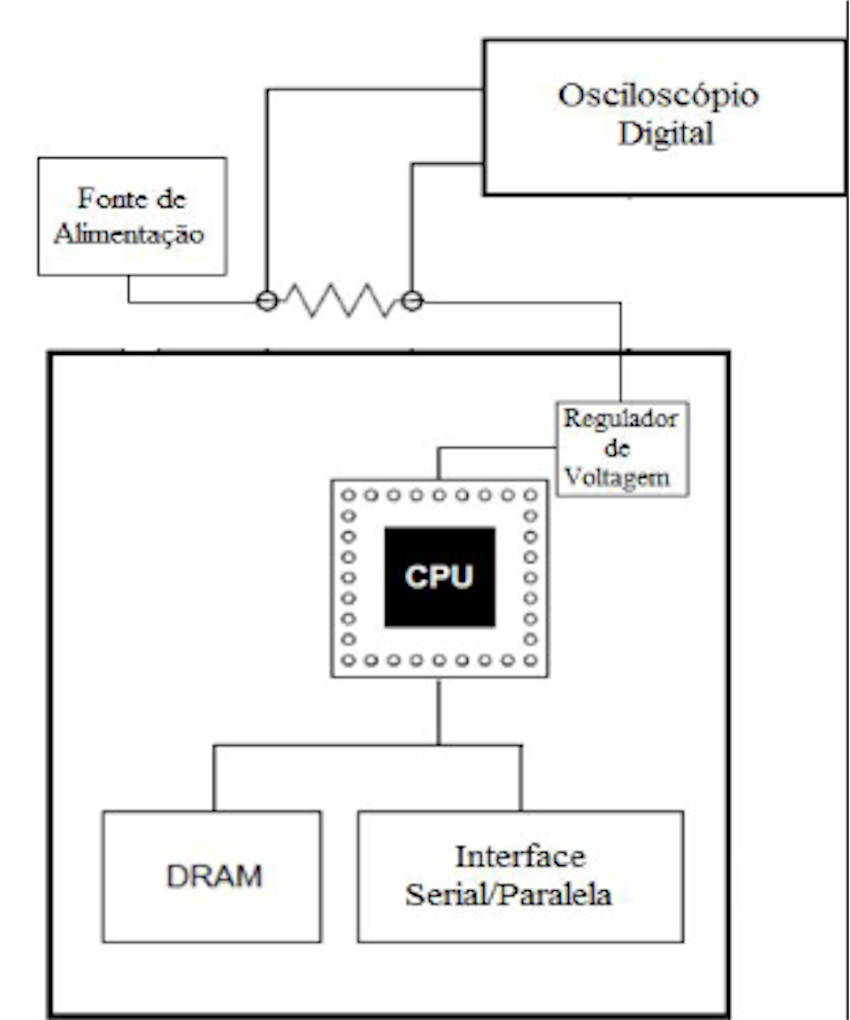
\includegraphics[scale=0.5]{images/ociloscopio.png}
    \caption{Figura 3 - Arquitetura da Plataforma. Retirado de (ALCANTARA; DE LIMA; FURTADO, 2019)}
    
\end{figure}
\end{itemize}   
\end{frame}
\begin{frame}{Fundamentação Teórica}
\begin{itemize}
    \item \textbf {Ripeto}\\  Ripeto, uma plataforma de avaliação para EHES que pode imitar o comportamento do transdutor de captação de energia e registrar em rastreamentos de energia de memória e dados do analisador lógico para assegurar adequadamente o desempenho de um EHES (ALCANTARA; DE LIMA; FURTADO, 2019). O Ripeto é baseado em um FPGA Sparten6, da Xilinx, com 32 Mb de memória de DRAM acoplada.
    \begin{figure}
        \centering
        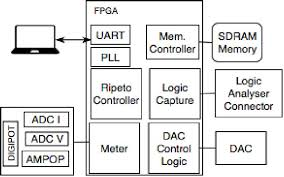
\includegraphics[scale=0.5]{images/ripeto.png}
        \caption{Figura 3 - Arquitetura da Plataforma. Retirado de (ALCANTARA; DE LIMA; FURTADO, 2019)}
        
    \end{figure}
\end{itemize}
\end{frame}


\section{Método Proposto}

\begin{frame}{Método Proposto}
  O  estudo  baseia-sefundamentalmente nos manuais dos fabricantes dos modelos dos microcontroladoresescolhidos  e  no  artigoAn FPGA-based evaluation platform for energy harvestingembedded systems(ALCANTARA;   DE   LIMA;   FURTADO,   2019)   para   fazer   osexperimentos.\\
  Para os experimentos, deverão ser realizada uma primeira etapa, onde ocorre umarevisão aprofundada o artigo anteriormente citado. Uma segunda, ondes os algoritmosserão implementados e testados.   Na terceira etapa,  o Repito será utilizado,  assimcomo o osciloscópio para se obter resultados quanto ao consumo energético. Por fim,na quarta etapa, com os resultados em mãos os perfis porão ser traçados com umaalta precisão.
 \end{frame}



\section{Cronograma}

\begin{frame}{Cronograma}

\begin{table}[!hp]
\centering
   \caption{Cronograma de pesquisa}

\begin{tabular}{|c|c|}
 
	\hline
	Mês &  O que será feito\\
	\hline
   1 &  Levantamento bibliografico e elaboração do projeto\\
	\hline
   2 &  Implementação de algoritmo\\
	\hline
	  3 &  Realização de experimentos\\
	\hline  
	4 & Realização de experimentos\\
	\hline  
	5 &  Coleta de dados e elaboração dos perfis de consum\\
	\hline
	  6 & Redação do trabalho, revisão e entraga da monografia\\
	\hline
	
\end{tabular}
\end{table}

\end{frame}


\section{Referências}

\begin{frame}{Referências}
CERQUEIRA, Marcos Vinícius Bião; COSTA, Daniel Gouveia. Um Modelo Matemático para Estimativas do Consumo de Energia em Redes de Sensores Visuais sem Fio. TEMA (São Carlos), v. 20, n. 2, p. 257-276, 2019.\\

DOS ANJOS LIMA, Felipe et al. Estudo do Consumo de Energia do Algoritmo Criptográfico AES no simulador da arquitetura ARM Sim-Panalyzer.\\

SANTOS NETO, Lealdo; MORENO, Edward David; BC DE MATOS, Leila. TÉCNICAS DE MEDIÇÃO DO CONSUMO DE ENERGIA EM PLATAFORMAS COMPUTACIONAIS. Revista de Sistemas e Computação-RSC, v. 1, n. 2, 2012.\\

ALCANTARA, Roberto Paulo Dias; DE LIMA, Otavio Alcantara; FURTADO, Corneli Gomes. An FPGA-based evaluation platform for energy harvesting embedded systems. In: 2019 32nd Symposium on Integrated Circuits and Systems Design (SBCCI). IEEE, 2019. p. 1-6.\\

\end{frame}
  


\end{document}
